%!TEX root = ../../main.tex

\subsection{Sensor Ø BDD}

\begin{figure}[H]
	\centering
	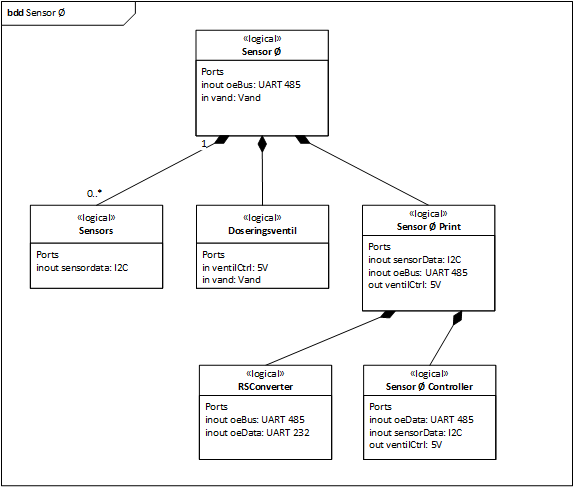
\includegraphics[width=0.82\textwidth]{Systemarkitektur/Sensoroe/Sensoroe_BDD.png}
	\label{fig:Sensoroe BDD}
	\caption{Block Definition Diagram af Sensor Ø}
\end{figure}

\subsubsection*{Sensor Ø Control}
Sensor Ø Control tager imod kommandoer fra KarControl, som instruerer omkring åbning og lukning af Doseringsventil. KarControl anmoder også om, at Sensor Ø Control skal sende måledata fra sensors, som er tilkoblet Sensor Ø’en.

\subsubsection{Doseringsventil}
Doseringsventilen åbner og lukker for vandtilførslen til planterne i området omkring Sensor Ø’en, som Doseringsventilen er tilkoblet. Når KarControl tænder for Vandpumpen kan de enkelte Sensor Ø’ers Doseringsventiler være åbne eller lukkede alt efter, om planterne omkring Sensor Ø’en har brug for vand.

\subsubsection{FieldSensor}
FieldSensor er en generalisering af alle slags sensorer, som kan tilsluttes Sensor Ø’en. Vilkårligt mange sensorer kan tilkobles en bus, og kommunikere med Sensor Ø Control gennem en standardiseret protokol. Sensor kan kun aflevere målinger når de bliver bedt om at levere dem.

\subsection{Sensor Ø IBD}

\begin{figure}[H]
	\centering
	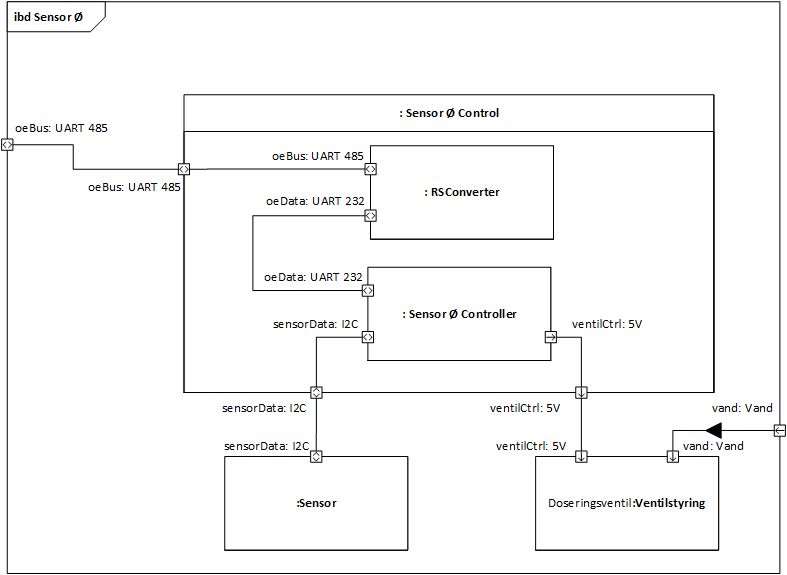
\includegraphics[width=0.82\textwidth]{Systemarkitektur/Sensoroe/Sensoroe_IBD.png}
	\label{fig:Sensoroe BDD}
	\caption{Internal Block Diagram af Sensor Ø}
\end{figure}

\begin{table}[H]
\centering
{\rowcolors{2}{white!80!black!30}{white!70!black!60} %farver på hver anden række -starter på 3
\setlength{\arrayrulewidth}{0.2mm}					 %tykkelse på linier 
\setlength{\tabcolsep}{10pt}						 %indryk i celle 
\renewcommand{\arraystretch}{1.5}					 %højden på tabelrum
\center
\begin{tabular}{|p{20mm}|p{40mm}|p{30mm}|p{30mm}|}		 %længden på alle rum
\hline

\multicolumn{4}{|>{\columncolor{white!20!black!90}}m{14.20cm}|}{\textcolor{white}{\large{\textbf{Signal beskrivelser}}}} \\\hline
\rowcolor{white!70!black!60}
\textcolor{black}{\large{\textbf{Navn}}}&
\textcolor{black}{\large{\textbf{Definition}}}&	
\textcolor{black}{\large{\textbf{Område}}}&
\textcolor{black}{\large{\textbf{Kommentar}}}\\
\hline
oeData				& buskommunikation efter konvertering fra 485 &	 	& UART kommunikation fra 485 bussen  \\
oeBus				& RS485 bus til kommunikation mellem enheder  &	 	& Differentielt bussystem  \\
sensorData			& Signal på I2C bus							  &	 	& Kan være flere forskellige signaler alt efter sensor type   \\
ventilCtrl			& Signal til styring af doserings ventil	  &	0-5V& Bruges til at styre mængden af vand til planterne \\
vand				& Dette er flow'et af vand 					  &		& \\
\hline
\end{tabular}
}
\caption{signal beskrivelser for KarControl}
\label{table:SignalBeskrivelserKarControl}
\end{table}

%\subsection{Sensoroe Allokeringsdiagram}
%
%\begin{figure}[H]
%	\centering
%	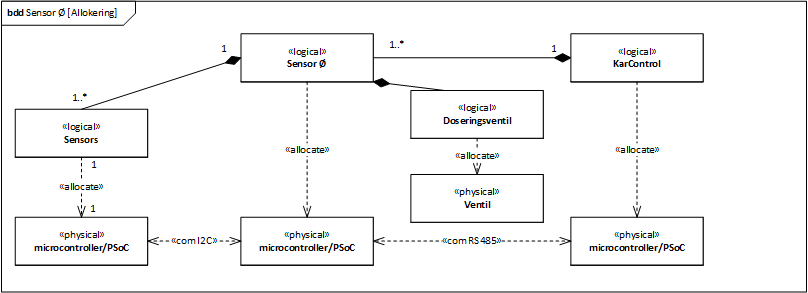
\includegraphics[width=0.82\textwidth]{Systemarkitektur/Sensoroe/Sensoroe_Allokeringsdiagram.png}
%	\label{fig:Sensoroe BDD}
%	\caption{Allokeringsdiagram af Sensoroe}
%\end{figure}